The model is trained with PyTorch 1.10.2, CUDA 10.2.89, GPU with single NVIDIA GEFORCE GTX 1080Ti.


%% nnn24 exp
\section{Neighbor Input}


%% nnnn exp
\section{Vertex Input}

%% resng
\section{ResNet+Gated Convolution}


%% nconv exp
\section{Normalized Convolution}










\section{Detail Enhance using Canny Edge Detector}


Figure \ref{fig:washington_gt_ngpred} shows the ground truth and predicted normal map of a Washington statue. In the predicted normal map, as shown on the right side, the relief on the side of stone chair is lack of sharpness compare to the ground truth on the left side. 
\begin{figure}[!h]
	\centering
	{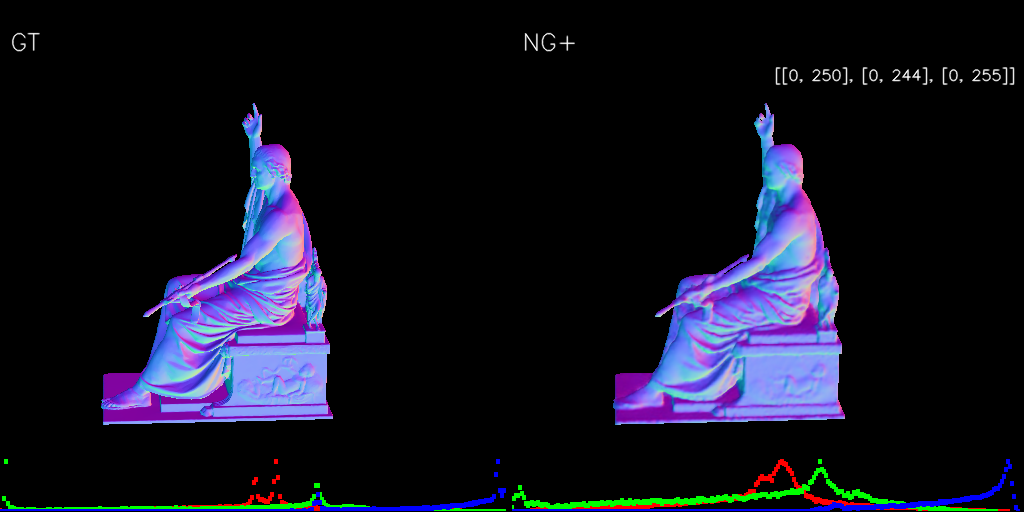
\includegraphics[width=\textwidth]{./pic/00349.gt.ngplus.png}}
	\label{fig:washington_gt_ngpred}
	\caption{Left: Ground truth normal map; Right: Predicted normal map based on model "NG"}
\end{figure}

To further visualize the error of predicted normal map, figure \ref{fig:canny_edge_details} shows the angle error of normal map. 
It is obvious to see, that the error goes higher in the coarse surface, like fingers, gown and relief. Oppositely, the error goes lower in the smooth surface, like the arm, face, and foot. The coarse surface are mainly the boundaries, or edges, which can be extract efficiently using edge detection algorithms, like Canny Edge detector. Figure \ref{fig:canny_edge_details} shows the detected edge of ground truth using Canny Edge Detector.

\begin{figure}[!h]
	\centering
	{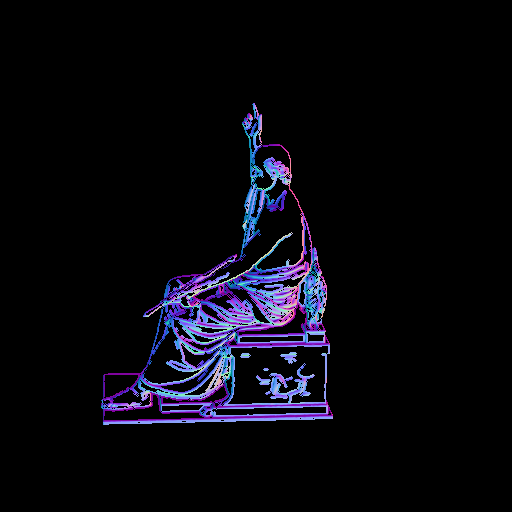
\includegraphics[width=0.45\textwidth]{./pic/00349.hpf0.png}}
	{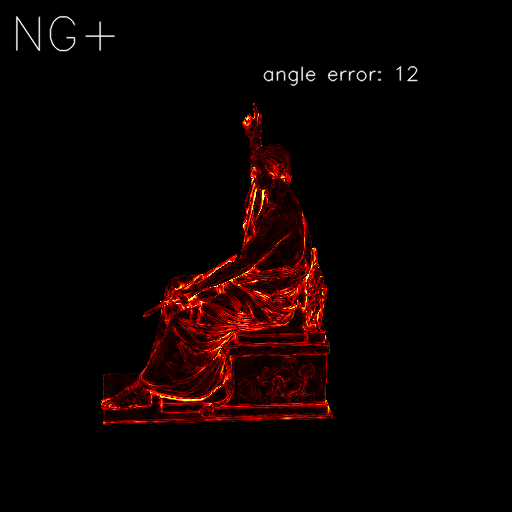
\includegraphics[width=0.45\textwidth]{./pic/00349.error.png}}
	\label{fig:canny_edge_details}
	\caption{Left: Normal Map; Middle: Detected Edge of Normal Map using Canny Edge Detection Algorithm; Right: Error of predicted normal map.}
\end{figure}